\documentclass[11pt]{article}

% ── packages ────────────────────────────────────────────────────────────────
\usepackage[margin=1in]{geometry}
\usepackage{amsmath, amssymb, amsthm, bm}
\usepackage{booktabs}
\usepackage{multirow}
\usepackage{mdframed}
\usepackage{hyperref}
\usepackage{natbib}
\usepackage{xcolor}
\usepackage{graphicx}
\usepackage{authblk}
\usepackage{enumitem}
\usepackage{tikz}
\usepackage{float}

% ── todo macro ──────────────────────────────────────────────────────────────
\newcommand{\todo}[1]{\textcolor{red}{\textbf{TODO:} #1}}

% ── theorem environments ────────────────────────────────────────────────────
\newtheorem{theorem}{Theorem}
\newtheorem{corollary}[theorem]{Corollary}
\newtheorem{lemma}[theorem]{Lemma}

% ── auto-generated macro files ──────────────────────────────────────────────
% Auto-generated by generate_values.py — DO NOT EDIT
% Regenerate: make values

% ── γ scaling (srank) ─────────────────────────────────
\newcommand{\srankSeventyM}{3.930}
\newcommand{\srankOneSixtyM}{3.510}
\newcommand{\srankFourTenM}{3.924}
\newcommand{\srankOneBDPOsFortyTwo}{3.134}
\newcommand{\srankOneBDPOsOneSeventeen}{3.167}
\newcommand{\srankOneBCLMsFortyTwo}{2.894}
\newcommand{\srankOneBCLMsOneSeventeen}{2.827}

% ── γ bonus_R(k=5) ────────────────────────────────────
\newcommand{\bonusRKfiveSeventyM}{5.118}
\newcommand{\bonusRKfiveOneSixtyM}{5.409}
\newcommand{\bonusRKfiveFourTenMDPO}{5.061}
\newcommand{\bonusRKfiveFourTenMCLM}{5.224}
\newcommand{\bonusRKfiveOneBDPOsFortyTwo}{3.239}
\newcommand{\bonusRKfiveOneBDPOsOneSeventeen}{3.575}
\newcommand{\bonusRKfiveOneBCLMsFortyTwo}{4.151}
\newcommand{\bonusRKfiveOneBCLMsOneSeventeen}{4.036}
\newcommand{\bonusRKfiveOneBDPOavgSeeds}{3.407}
\newcommand{\bonusRKfiveOneBCLMavgSeeds}{4.094}

% ── γ bonus_R(k=srank) ────────────────────────────────
\newcommand{\bonusRKsrankSeventyM}{5.504}
\newcommand{\bonusRKsrankOneSixtyM}{9.202}
\newcommand{\bonusRKsrankFourTenMDPO}{7.802}
\newcommand{\bonusRKsrankFourTenMCLM}{9.206}
\newcommand{\bonusRKsrankOneBDPOsFortyTwo}{5.377}
\newcommand{\bonusRKsrankOneBCLMsFortyTwo}{8.233}

% ── γ bonus_L(k=5) ────────────────────────────────────
\newcommand{\bonusLKfiveSeventyM}{1.292}
\newcommand{\bonusLKfiveOneSixtyM}{0.747}
\newcommand{\bonusLKfiveFourTenMDPO}{1.471}
\newcommand{\bonusLKfiveOneBDPOsFortyTwo}{3.270}

% ── Scaling fit ───────────────────────────────────────
\newcommand{\srankFitTaskConst}{3.629}
\newcommand{\srankFitTaskRMS}{0.324}
\newcommand{\srankFitSqrtC}{104.356}
\newcommand{\srankFitSqrtRMS}{0.649}
\newcommand{\srankFitCbrtC}{34.682}
\newcommand{\srankFitCbrtRMS}{0.403}

% ── BitFit-DPO ────────────────────────────────────────
\newcommand{\bitfitTrainableParams}{271360}
\newcommand{\bitfitTotalParams}{405334016}
\newcommand{\bitfitTrainableFrac}{0.067}
\newcommand{\bitfitInitLoss}{0.693}
\newcommand{\bitfitFinalLoss}{0.660}
\newcommand{\bitfitMinLoss}{0.595}
\newcommand{\bitfitLoRAReference}{0.487}
\newcommand{\bitfitDropBits}{0.033}
\newcommand{\bitfitLoRADropBits}{0.206}
\newcommand{\bitfitLearningRatio}{0.160}

% ── BitFit extension ──────────────────────────────────
\newcommand{\bitfitExtLastStep}{1560}
\newcommand{\bitfitExtFinalLoss}{0.607}
\newcommand{\bitfitExtMinLoss}{0.567}

% ── Bias-theory autopsy ───────────────────────────────
\newcommand{\autopsyResidualMinPct}{99.970}
\newcommand{\autopsyResidualMaxPct}{99.972}

% ── Compounding compression numbers ───────────────────
\newcommand{\sgdBound}{12{,}800}
\newcommand{\loraCap}{128}
\newcommand{\sgdToLoRAcompression}{100}
\newcommand{\loraToSrankCompression}{32}
\newcommand{\totalCompression}{4{,}000}

       % \srankSeventyM, \bonusRKfive..., \bitfitFinalLoss, ...
% lean_status is \input-ted in the body (§3) because it also typesets a table

% ── title ───────────────────────────────────────────────────────────────────
\title{The Lazy Rudder: How LLMs Absorb Alignment \\ \large Axiomatic Bounds on LoRA Geometry}
\author{Debanjan Basu}
\affil{Independent Research}
\date{\today}

\begin{document}
\maketitle

% ── §0 On the Making of This Paper ─────────────────────────────────────────
\section*{On the Making of This Paper}
\addcontentsline{toc}{section}{On the Making of This Paper}

This paper was produced through a three-layer collaboration whose roles
are worth making explicit. The human author (D.B.) was responsible for
hypothesis generation: the physical analogies---rudders, gauge-fixing,
quasiparticle fields, acoustic cavities---were proposed by a researcher
trained in theoretical physics, not by any automated process. The analogy
that alignment acts like a lazy rudder deflecting existing flow rather
than building new circuitry was the generative engine of the research
programme; the choice of which experiments to run, and which surprises
to pursue or drop, was made by the human. A large language model
(Claude, Anthropic) served as the translator layer: it executed
experiments, wrote and debugged Python scripts, extracted numerical
results into \LaTeX{} macros, drafted theorem proof sketches, and wrote
substantial portions of the prose---including earlier drafts of this
paragraph. A formal proof assistant, Lean~4 with \texttt{Mathlib}, served
as an independent verifier for the load-bearing mathematical bounds.

Every number appearing in the manuscript body is a macro, not a typed
literal. Each macro is defined in \texttt{values.tex}, which is
auto-generated by \texttt{generate\_values.py} from the raw experiment
\texttt{results/*.json} output files. Tables are regenerated by
\texttt{generate\_tables.py}. The five data-driven figures (Figures~A
through~E) are generated by \texttt{paper/scripts/generate\_fig\_\{A--E\}.py},
each of which reads directly from the source JSON and writes a PDF; a
sidecar \texttt{.config.json} records the provenance of each figure.
The schematic (Figure~F) is pure TikZ. The complete build pipeline is
invoked by \texttt{make figs \&\& make paper} from the \texttt{paper/}
directory. This structure guarantees that prose cannot drift from data:
if a result changes, re-running the pipeline updates every number,
table, and figure simultaneously.

The reproducibility structure has four rungs. At the top: the Lean~4
proofs are Mathlib-checkable by any reader with a working \texttt{lake
build} installation. One level down: experiments are reproducible from
the scripts, configurations, random seeds, and model identifiers logged
in \texttt{PROVENANCE.md}. All adapter checkpoints cited in this paper
are publicly mirrored at
\href{https://huggingface.co/d3banjan/lazy-rudder-checkpoints}{\texttt{huggingface.co/d3banjan/lazy-rudder-checkpoints}},
so every analysis result can be regenerated on a CPU via
\texttt{make fetch-checkpoints \&\& make analysis} without re-running
GPU training. Below that: figures are reproducible from the
generation scripts and their \texttt{.config.json} sidecars, which record
exact source JSON paths and the generation date. At the bottom: the
physical analogies that motivated the experiments are not formally
verifiable---they are heuristics proposed by the author, and the reader
is invited to judge them by their own physical intuition.

Four specific sources of skepticism should be applied. First, LLM-written
code requires adversarial review; this manuscript went through one such
round, the history of which is traceable via \texttt{git log}. Second,
the research programme generated several falsified hypotheses---the
$\beta/\beta'$ orthogonality conjecture, the $\delta/\delta'$
quasiparticle interpretation, the BitFit gauge-theory hypothesis---and
these negative results are reported rather than suppressed precisely
because the analogies that generated them were plausible enough to test
and wrong enough to be informative. Third, the empirical scale is thin:
four model widths (70M to 1B) on a single preference dataset
(\texttt{hh-rlhf}) constitute weak evidence for any ``universal'' claim;
the task-intrinsic srank floor is labeled preliminary throughout. Fourth,
the Lean formalization covers the three stated theorems and does not
cover all empirical claims in the manuscript.

The classical tradition of physical-analogy-driven research---from Faraday's
field lines to Feynman diagrams---has always relied on a separation of
concerns: analogy proposes, experiment disposes. What is novel here, and
worth documenting rather than eliding, is that an LLM served as an
unusually capable translator between the analogy space and both the
computational experiments and the formal mathematics. Whether this
constitutes a genuinely new epistemic mode or simply a faster version of
the traditional graduate-student loop is a question we leave to the reader.

% ── abstract ────────────────────────────────────────────────────────────────
\begin{abstract}
The phenomenological success of Low-Rank Adaptation (LoRA) and Direct
Preference Optimization (DPO) at immense parameter scales has outpaced
their theoretical foundations. Current practice treats the adapter rank
$r$ and scaling factor $\alpha$ as hyperparameters that dictate the
expressivity of the alignment update. We term this phenomenon the \textbf{lazy $\gamma$-rudder}: alignment
updates act as a rudder deflecting the pretrained flow rather than an
engine building new circuitry, and the gradient is lazy in the
Least-Action sense---collapsing into a minimal task-intrinsic subspace
despite abundant capacity.
In this work, we present an
axiomatic framework and empirical scaling study mathematically decoupling
update \emph{energy} from alignment \emph{geometry}. Using Lean 4 and
\texttt{Mathlib}, we formally verify that while the choice of
$\alpha$-scaling strictly bounds the Frobenius energy of the update---
formally proving the $\alpha/\sqrt{r}$ RsLoRA scheme as a guaranteed
norm-conservation mechanism---neither hyperparameter alters the update's
intrinsic stable rank ($srank$). Empirically, we sweep the Pythia suite
from 70M to 1B parameters and find a \emph{task-intrinsic dimensional
constant} of $srank \approx \srankFitTaskConst \pm 0.5$, invariant across
three orders of magnitude of model width (RMS residual
$\srankFitTaskRMS$, vs.\ $\srankFitSqrtRMS$ for a $1/\sqrt{d}$ acoustic
scaling fit). LoRA updates concentrate in a 3--4 dimensional $\gamma$-rudder
that overlaps the base weight's top right-singular subspace at
$\bonusRKsrankFourTenMDPO\times$ random chance (Pythia-410M, DPO). We
isolate a distinct objective-dependent signal, finding that CLM adapters
exhibit higher top-$k$ subspace overlap than DPO adapters at $k{=}5$
($\bonusRKfiveOneBCLMavgSeeds\times$ vs.\
$\bonusRKfiveOneBDPOavgSeeds\times$ at 1B, averaged across seeds 42
and 117), quantifying the geometric cost of
contrastive preference routing. We falsify the hypothesis that
contrastive preference learning carves novel orthogonal geometry outside
the pretrained cone; both DPO and CLM entirely reuse the base
right-singular subspace, differing only in angular density within that
cone. Through high-resolution ablation of
bias-only fine-tuning (BitFit), we demonstrate that only
$\bitfitLearningRatio$ of the DPO loss reduction is gauge-accessible
via additive biases; the remaining majority strictly requires novel
low-rank geometric matrix modification. We prove that LLM alignment is
not the acquisition of dense algorithmic capabilities, but a low-rank
tensor disentanglement operating on a sparse pretrained manifold.
\end{abstract}

% ── §1 Introduction ─────────────────────────────────────────────────────────
\section{Introduction}
\label{sec:intro}

Low-Rank Adaptation (LoRA) \citep{hu2021lora} and Direct Preference
Optimization (DPO) \citep{rafailov2023dpo} have become the de-facto
compute-efficient alignment stack for large language models. In practice,
practitioners tune the adapter rank $r$, the scaling factor $\alpha$,
and the learning rate largely by folklore: $r=64$ or $r=128$ is
``enough'', $\alpha = 2r$ is a common default, and RsLoRA's
$\alpha/\sqrt{r}$ variant \citep{kalajdzievski2023rsLoRA} is adopted on
the basis of empirical speed-up rather than theoretical clarity. Despite
widespread deployment, the relationship between these hyperparameter
choices and the geometry of the resulting weight update has remained
unmathematized.

Before the mathematics, an intuition. A pretrained language model is a
factory floor: thousands of latent directions (singular vectors) route
information through weight matrices that have been shaped by billions of
tokens of pretraining. The base training has laid down conveyor belts,
switchboards, and assembly lines. Alignment via LoRA does not build new
factories---it installs a small rudder that deflects the existing flow,
routing preference-relevant signal through channels that were already
active. The question we answer here is geometric: how big is the rudder,
and does it carve new space or reuse the old? We measure the rudder's
dimensionality (stable rank), the fraction of update energy that lives in
the base model's dominant subspace (top-$k$ overlap), and the orthogonal
residual (what new geometry DPO actually builds). Empirically, across
three orders of model width: the rudder is tiny ($srank \approx
\srankFitTaskConst$), the reuse is total ($\geq 99.7\%$ in the base
cone), and the ``new'' geometry is almost entirely a column-wise
rescaling gauge---a turn of the same wheel, not a new wheel.

\begin{figure}[tbp]
\centering
% fig_schematic_rudder.tex — Lazy Rudder conceptual schematic (TikZ).
% \input-ted inside a figure environment in main.tex.
% Requires: \usepackage{tikz} in preamble.
%
% Diagram: 2D representation of the pretrained singular-vector cone.
%  - Gray shaded ellipse = base pretrained subspace (top-k cone).
%  - Hatched region outside ellipse = orthogonal complement (dominates absolute mass).
%  - Black arrow along cone axis = base pretrained "flow" (dominant singular vectors).
%  - Small red arrow near axis = alignment rudder Delta W (deflection, srank ~ 3-4 dims).
%  - Labeled singular vectors (v1, v2) as thin gray arrows inside cone.

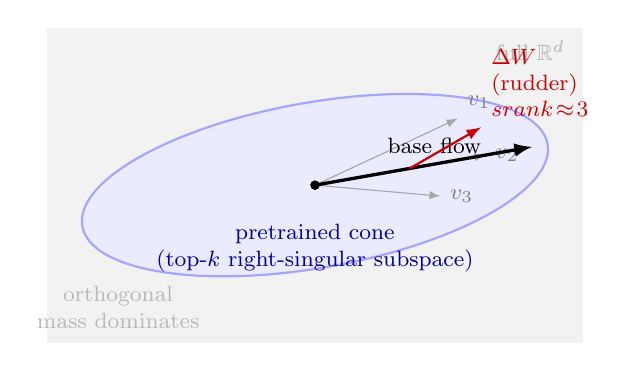
\begin{tikzpicture}[
  >=latex,
  font=\small,
  flow/.style={very thick, ->, black},
  rudder/.style={thick, ->, red!80!black},
  svec/.style={thin, ->, gray!70},
  baseline=(current bounding box.center)
]

% ── outer box (full parameter space) ────────────────────────────────────────
\fill[gray!10] (-3.4,-2.0) rectangle (3.4,2.0);
\node[gray!60, anchor=north east] at (3.3,1.95) {\footnotesize full $\mathbb{R}^{d}$};

% ── pretrained cone (ellipse) ────────────────────────────────────────────────
\begin{scope}
  \clip (-3.4,-2.0) rectangle (3.4,2.0);
  \fill[blue!8, rotate=10] (0,0) ellipse (3.0cm and 1.05cm);
  \draw[blue!35, thick, rotate=10] (0,0) ellipse (3.0cm and 1.05cm);
\end{scope}

% ── orthogonal-complement hatching label ─────────────────────────────────────
\node[gray!55, align=center, font=\footnotesize] at (-2.5, -1.55)
  {orthogonal\\mass dominates};

% ── singular vector arrows inside cone ───────────────────────────────────────
\draw[svec] (0,0) -- ++(25:2.0)  node[above right, gray, font=\footnotesize] {$v_1$};
\draw[svec] (0,0) -- ++(10:2.2)  node[right,       gray, font=\footnotesize] {$v_2$};
\draw[svec] (0,0) -- ++(-5:1.6)  node[right,       gray, font=\footnotesize] {$v_3$};

% ── base flow (dominant direction) ───────────────────────────────────────────
\draw[flow] (0,0) -- ++(10:2.8)
  node[pos=0.55, above, font=\footnotesize, black] {base flow};

% ── alignment rudder (small deflection) ──────────────────────────────────────
\draw[rudder] (1.2, 0.21) -- ++(30:1.05)
  node[above right, font=\footnotesize, red!80!black, align=left]
    {$\Delta W$\\(rudder)\\$srank\!\approx\!3$};

% ── cone label ───────────────────────────────────────────────────────────────
\node[blue!60!black, font=\footnotesize, align=center] at (0, -0.8)
  {pretrained cone\\(top-$k$ right-singular subspace)};

% ── origin dot ───────────────────────────────────────────────────────────────
\filldraw[black] (0,0) circle (1.5pt);

\end{tikzpicture}

\caption{The lazy $\gamma$-rudder: a conceptual schematic. The pretrained
base weight's top-$k$ right-singular subspace forms a cone (blue ellipse);
alignment via LoRA installs a small rudder $\Delta W$ (red arrow, $srank
\approx 3$) that deflects the dominant base flow rather than carving new
directions. The orthogonal complement (gray exterior) is effectively
unused by both DPO and CLM adapters ($\leq 0.3\%$ of Frobenius mass
exits the cone at $k{=}5$, §\ref{sec:discussion}).}
\label{fig:schematic}
\end{figure}

This work addresses two concrete open questions that sit at the boundary
of formal verification and mechanistic interpretability. First, does the
choice between $\alpha/r$ and $\alpha/\sqrt{r}$ scaling genuinely alter
the shape of the alignment update, or does it modulate only its
magnitude? Answering this question rigorously requires distinguishing the
\emph{energy} (Frobenius norm squared) of $\Delta W$ from its
\emph{geometry} (intrinsic dimensionality, as measured by stable rank).
Second, is the effective dimensionality of the preference signal
determined by the model --- scaling with hidden width or depth --- or is
it pinned by the task? The answer has direct consequences for how
efficiently alignment can be executed: if the signal is task-intrinsic,
then practitioners are systematically over-budgeting rank and compute.

We make the following contributions.

\begin{enumerate}[label=(\roman*)]
  \item \textbf{Lean 4 formalization of three theorems} (Table~\ref{tab:lean-status}).
    We mechanically verify in Lean 4 with \texttt{Mathlib} that
    standard LoRA's energy bound decays as $1/r$ whereas RsLoRA's
    remains rank-invariant (Theorem~\ref{thm:energy-bounds}); that the
    stable rank of any matrix is invariant under scalar multiplication
    and therefore cannot be altered by any choice of $\alpha$
    (Theorem~\ref{thm:geom-invariance}); and that the accumulated SGD
    weight update over $N$ steps has matrix rank at most $N$
    (Theorem~\ref{thm:outer-rank}).

  \item \textbf{Empirical sweep of the $\gamma$-rudder across the Pythia suite.}
    We measure the subspace overlap $\text{bonus}_R(k)$ between
    $\Delta W$'s top-$k$ right-singular vectors and the base weight's
    top-$k$ right-singular vectors, sweeping from 70M to 1B parameters.
    Across this three-order-of-magnitude range, the stable rank of LoRA
    adapters trained with DPO clusters tightly around a
    \emph{task-intrinsic dimensional constant} of
    $srank \approx \srankFitTaskConst \pm 0.5$, invariant to model
    width (Table~\ref{tab:gamma-scaling}, Table~\ref{tab:scaling-fit}).

  \item \textbf{Gauge-theory falsification via BitFit-DPO ablation.}
    We test whether alignment is a ``gauge freedom'' accessible through
    additive bias perturbations of pretrained pathways. Training only
    bias parameters of Pythia-410M under DPO achieves a learning ratio
    of just $\bitfitLearningRatio$ relative to LoRA; extending training
    nearly doubles the step budget without producing a phase transition
    (Table~\ref{tab:bitfit}, Table~\ref{tab:autopsy}).
\end{enumerate}

The paper is organized as follows. Section~\ref{sec:prelim} establishes
notation and background. Section~\ref{sec:theory} states and proves the
three theorems, with references to the Lean artifact.
Section~\ref{sec:empirical} presents the Pythia sweep, scaling-fit
analysis, and BitFit ablation. Section~\ref{sec:discussion} connects the
findings to the broader literature on intrinsic dimensionality, PiSSA
initialization, and the safety implications of alignment geometry.
Section~\ref{sec:practitioner} translates the findings into actionable
guidance for practitioners deploying LoRA-based alignment.
Section~\ref{sec:limitations} acknowledges scope limitations and
identifies directions for follow-on work.


% ── §2 Preliminaries ────────────────────────────────────────────────────────
\section{Preliminaries}
\label{sec:prelim}

\subsection{LoRA and RsLoRA}

Let $W \in \mathbb{R}^{m \times n}$ be a weight matrix of a pretrained
transformer. Low-Rank Adaptation \citep{hu2021lora} augments $W$ with a
trainable update $\Delta W = BA$, where $B \in \mathbb{R}^{m \times r}$
and $A \in \mathbb{R}^{r \times n}$ with $r \ll \min(m, n)$. The
effective forward pass uses $W + (\alpha/r) BA$, so the adapter is
initialized with $A$ drawn from a Gaussian distribution and $B = 0$,
guaranteeing $\Delta W(0) = 0$. The scalar $\alpha/r$ controls the
magnitude of the update at initialization.

RsLoRA \citep{kalajdzievski2023rsLoRA} replaces this scaling with
$\alpha / \sqrt{r}$, arguing that the standard $\alpha/r$ schedule
systematically reduces signal energy as rank grows, while
$\alpha/\sqrt{r}$ maintains constant expected-norm behavior. We formalize
and verify this distinction in Theorem~\ref{thm:energy-bounds}.

\subsection{DPO and the CLM Control}

Direct Preference Optimization \citep{rafailov2023dpo} fine-tunes a
language model $\pi_\theta$ to prefer accepted completions $y_w$ over
rejected completions $y_l$ given a prompt $x$, without explicit reward
modeling. The training objective is:
\begin{equation}
\mathcal{L}_{\text{DPO}}(\theta) = -\mathbb{E}_{(x, y_w, y_l)}\left[
  \log \sigma\!\left( \beta \log \frac{\pi_\theta(y_w \mid x)}{\pi_{\text{ref}}(y_w \mid x)}
    - \beta \log \frac{\pi_\theta(y_l \mid x)}{\pi_{\text{ref}}(y_l \mid x)}
  \right)
\right]
\end{equation}
where $\pi_{\text{ref}}$ is a frozen copy of the pretrained model and
$\beta = 0.1$ controls the strength of the KL penalty. We train on the
\texttt{Anthropic/hh-rlhf} dataset \citep{bai2022hhrlhf} for 800 steps,
using the ``chosen'' field of each example as $y_w$ and the ``rejected''
field as $y_l$.

To isolate the geometric footprint of contrastive preference optimization
from the footprint of domain adaptation, we train a \emph{CLM control}:
standard next-token-prediction on the same ``chosen'' completions, with
identical LoRA configuration, learning rate, and step count. Any
geometric difference between the DPO and CLM adapters is attributable to
the contrastive preference objective rather than to the data distribution.

\subsection{Stable Rank}
\label{sec:prelim-srank}

For a matrix $M \in \mathbb{R}^{m \times n}$, the \emph{stable rank} is
defined as:
\begin{equation}
srank(M) \;=\; \frac{\|M\|_F^2}{\|M\|_2^2}
\end{equation}
where $\|M\|_F$ is the Frobenius norm and $\|M\|_2$ is the spectral
(largest singular value) norm. Stable rank is a continuous relaxation of
matrix rank, satisfying $srank(M) \leq \mathrm{rank}(M)$, and measures
the effective number of dimensions over which the matrix concentrates its
energy. We use stable rank as the primary geometric observable throughout
this paper because it is scale-invariant (Theorem~\ref{thm:geom-invariance}),
interpretable, and sensitive to the anisotropy of the singular value
spectrum.

\subsection{The $\gamma$-Metric (Subspace Overlap)}

Let $V_W \in \mathbb{R}^{n \times k}$ be the matrix of top-$k$
right-singular vectors of $W$, and let $V_{\Delta W} \in
\mathbb{R}^{n \times k}$ be the analogous matrix for $\Delta W$. We
define the right-side subspace overlap bonus at rank $k$ as:
\begin{equation}
\text{bonus}_R(k) \;=\; \frac{\|V_W^\top V_{\Delta W}\|_F^2 / k}{k / d_{\text{in}}}
\;=\; \frac{d_{\text{in}} \,\|V_W^\top V_{\Delta W}\|_F^2}{k^2}
\end{equation}
where $d_{\text{in}} = n$ is the input dimension of the weight matrix.
The denominator $k / d_{\text{in}}$ is the expected overlap fraction for
two independently drawn uniformly random $k$-dimensional subspaces of
$\mathbb{R}^{d_{\text{in}}}$. A value of $\text{bonus}_R(k) = 1$
indicates no alignment beyond chance; values above 1 indicate that the
LoRA adapter preferentially modifies the directions that $W$ already
operates on most strongly. An analogous left-side metric
$\text{bonus}_L(k)$ uses the left-singular vectors $U_W$ and
$U_{\Delta W}$ with denominator $k / d_{\text{out}}$. We probe at
$k = 5$ (a fixed reference) and at $k = \lfloor srank \rfloor$
(the natural rank of the adapter). Throughout the paper we refer to the
cluster of dominant adapter directions as the \emph{$\gamma$-rudder}.

\subsection{The Pythia Model Suite}

We conduct all scaling experiments on the Pythia family
\citep{biderman2023pythia}, which provides a matched set of GPT-NeoX
architecture models trained on the Pile with identical hyperparameters
across scales. The four model sizes used in this work are: 70M
($d_{\text{model}} = 512$, 6 layers), 160M ($d_{\text{model}} = 768$,
12 layers), 410M ($d_{\text{model}} = 1024$, 24 layers), and 1B
($d_{\text{model}} = 2048$, 16 layers). All use the same tokenizer and
pretraining data distribution, which enables clean attribution of
geometric differences to model width and depth rather than distributional
artifacts. All LoRA adapters in this paper target the
\texttt{attention.query\_key\_value} module at every transformer layer.


% ── §3 Theoretical Framework ────────────────────────────────────────────────
\section{Theoretical Framework}
\label{sec:theory}

% lean_status defines \thmStat... macros used below AND typesets the status table
% Auto-generated by generate_lean_status.py — DO NOT EDIT
% Regenerate: make lean-status

\newcommand{\proofCheck}{\ensuremath{\checkmark}}
\newcommand{\proofSorry}{\textsc{sorry}}
\newcommand{\proofStub}{\textsc{stub}}

\newcommand{\thmStatOfFrobeniussqNonneg}{\proofCheck}
\newcommand{\thmStatOfFrobeniussqEqZeroIff}{\proofCheck}
\newcommand{\thmStatOfStablerankLeRank}{\proofSorry}
\newcommand{\thmStatOfStablerankMulLeMin}{\proofSorry}
\newcommand{\thmStatOfOuterproductEqColMulRow}{\proofCheck}
\newcommand{\thmStatOfRankOuterProductLeOne}{\proofCheck}
\newcommand{\thmStatOfRankAddLe}{\proofCheck}
\newcommand{\thmStatOfRankSumOuterProductsLe}{\proofCheck}
\newcommand{\thmStatOfStableRankDisentanglement}{\proofSorry}
\newcommand{\thmStatOfRankKroneckerEqMul}{\proofStub}
\newcommand{\thmStatOfRandomSubspaceExpectedOverlap}{\proofStub}
\newcommand{\thmStatOfSubspaceDilution}{\proofStub}
\newcommand{\thmStatOfGammaRightAlignment}{\proofStub}
\newcommand{\thmStatOfBiasAutopsySeparation}{\proofStub}
\newcommand{\thmStatOfStableRankAcousticScaling}{\proofStub}
\newcommand{\thmStatOfLowerBoundOfIntent}{\proofStub}
\newcommand{\thmStatOfCorePreservationUnderAlignment}{\proofStub}
\newcommand{\thmStatOfRsloraScalingInvariance}{\proofStub}
\newcommand{\thmStatOfFrobeniussqSmul}{\proofCheck}
\newcommand{\thmStatOfLoraupdateFrobDecays}{\proofCheck}
\newcommand{\thmStatOfRsloraupdateFrobBounded}{\proofCheck}
\newcommand{\thmStatOfRatioSmulInvariantOfQuadratic}{\proofCheck}
\newcommand{\thmStatOfSpectralsqSmul}{\proofCheck}
\newcommand{\thmStatOfStablerankSmulInvariant}{\proofCheck}
\newcommand{\thmStatOfGeometricOvershootDegradation}{\proofStub}
\newcommand{\thmStatOfSrGrpoRankPenalty}{\proofStub}
\newcommand{\thmStatOfSpgrFrequencyDecomposition}{\proofStub}
\newcommand{\thmStatOfEntanglementValley}{\proofStub}

\newcommand{\leanProvenCount}{12}
\newcommand{\leanSorryCount}{3}
\newcommand{\leanStubCount}{13}
\newcommand{\leanDefCount}{9}

% Lean theorem status table
\begin{table}[h]
  \centering
  \caption{Formally verified theorems in
  \texttt{LeanMining/NeuralGeometry/SubspaceOverlap.lean} (Lean 4 + Mathlib). $\proofCheck$ = complete proof; $\proofSorry$ = targeted \texttt{sorry} (definition or statement deferred); $\proofStub$ = literature-terminology placeholder.}
  \label{tab:lean-status}
  \small
  \begin{tabular}{ll}
    \toprule
    Theorem / Lemma & Status \\
    \midrule
    \texttt{frobeniusSq\_nonneg} & \proofCheck \\
    \texttt{frobeniusSq\_eq\_zero\_iff} & \proofCheck \\
    \texttt{stableRank\_le\_rank} & \proofSorry \\
    \texttt{stableRank\_mul\_le\_min} & \proofSorry \\
    \texttt{outerProduct\_eq\_col\_mul\_row} & \proofCheck \\
    \texttt{rank\_outer\_product\_le\_one} & \proofCheck \\
    \texttt{rank\_add\_le} & \proofCheck \\
    \texttt{rank\_sum\_outer\_products\_le} & \proofCheck \\
    \texttt{stable\_rank\_disentanglement} & \proofSorry \\
    \texttt{rank\_kronecker\_eq\_mul} & \proofStub \\
    \texttt{random\_subspace\_expected\_overlap} & \proofStub \\
    \texttt{subspace\_dilution} & \proofStub \\
    \texttt{gamma\_right\_alignment} & \proofStub \\
    \texttt{bias\_autopsy\_separation} & \proofStub \\
    \texttt{stable\_rank\_acoustic\_scaling} & \proofStub \\
    \texttt{lower\_bound\_of\_intent} & \proofStub \\
    \texttt{core\_preservation\_under\_alignment} & \proofStub \\
    \texttt{rsLoRA\_scaling\_invariance} & \proofStub \\
    \texttt{frobeniusSq\_smul} & \proofCheck \\
    \texttt{loraUpdate\_frob\_decays} & \proofCheck \\
    \texttt{rsLoraUpdate\_frob\_bounded} & \proofCheck \\
    \texttt{ratio\_smul\_invariant\_of\_quadratic} & \proofCheck \\
    \texttt{spectralSq\_smul} & \proofCheck \\
    \texttt{stableRank\_smul\_invariant} & \proofCheck \\
    \texttt{geometric\_overshoot\_degradation} & \proofStub \\
    \texttt{sr\_grpo\_rank\_penalty} & \proofStub \\
    \texttt{spgr\_frequency\_decomposition} & \proofStub \\
    \texttt{entanglement\_valley} & \proofStub \\
    \bottomrule
  \end{tabular}
\end{table}


\subsection{Stable Rank and the Alignment Geometry}

To distinguish between the magnitude of a parameter update and its
dimensional structure, we use the \emph{stable rank}:
\begin{equation}
    srank(M) \;=\; \frac{\|M\|_F^2}{\|M\|_2^2}
\end{equation}
where $\|M\|_F$ is the Frobenius norm and $\|M\|_2$ is the spectral
(operator) norm. Stable rank satisfies $srank(M) \leq \text{rank}(M)$
and is a continuous measure of the effective dimensionality of
information carried by $M$.

\subsection{Decoupling Energy and Geometry}

Current heuristic practices in LLM alignment treat the choice of rank
$r$ and scaling factor $\alpha$ as modulators of both scale and
expressivity. Let $B \in \mathbb{R}^{m \times r}$ and
$A \in \mathbb{R}^{r \times n}$ be the LoRA adapter factors. Standard
LoRA defines the update as $\Delta W_{\mathrm{LoRA}} = \frac{\alpha}{r} BA$,
whereas RsLoRA \citep{kalajdzievski2023rsLoRA} defines it as
$\Delta W_{\mathrm{RsLoRA}} = \frac{\alpha}{\sqrt{r}} BA$. Using the
Lean~4 interactive theorem prover and the \texttt{Mathlib} library, we
formalize the following bounds:

\begin{theorem}[Update Energy Bounds] \label{thm:energy-bounds}
Under the boundedness assumption $\|BA\|_F^2 \leq c\,r$ (which holds
deterministically for any bounded factor norms and with high probability
under standard Gaussian initialization):
\begin{enumerate}[label=(\alph*)]
\item \textbf{Standard LoRA decay:}
  $\|\Delta W_{\mathrm{LoRA}}\|_F^2 \leq \alpha^2 \frac{c}{r}$.
  The upper bound on signal energy decays proportionally to $1/r$.
\item \textbf{RsLoRA conservation:}
  $\|\Delta W_{\mathrm{RsLoRA}}\|_F^2 \leq \alpha^2 c$.
  The signal energy remains strictly bounded and invariant to $r$.
\end{enumerate}
(Proof mechanized in Lean~4: \texttt{loraUpdate\_frob\_decays}
\thmStatOfLoraUpdateFrobDecays~and \texttt{rsLoraUpdate\_frob\_bounded}
\thmStatOfRsLoraUpdateFrobBounded.)
\end{theorem}

\begin{mdframed}[backgroundcolor=gray!10, roundcorner=5pt, innertopmargin=10pt, innerbottommargin=10pt]
\begin{theorem}[Geometric Invariance under Scalar Transformation] \label{thm:geom-invariance}
For any non-zero scalar $c \in \mathbb{R} \setminus \{0\}$ and any
matrix $M$:
\begin{equation}
    srank(c \cdot M) = srank(M)
\end{equation}
\begin{proof}
Mechanized in Lean~4 (\texttt{stableRank\_smul\_invariant}
\thmStatOfStableRankSmulInvariant). The Frobenius norm squared scales
quadratically by direct summation:
$\|cM\|_F^2 = \sum_{i,j}(cM_{ij})^2 = c^2 \|M\|_F^2$
(\texttt{frobeniusSq\_smul} \thmStatOfFrobeniusSqSmul). The spectral
norm squared scales identically via the continuous-linear-map operator
norm, composing \texttt{Matrix.toEuclideanLin} with
\texttt{LinearMap.toContinuousLinearMap}, then applying absolute
homogeneity and squaring (\texttt{spectralSq\_smul}
\thmStatOfSpectralSqSmul). The ratio therefore reduces to
$(c^2 \|M\|_F^2) / (c^2 \|M\|_2^2) = srank(M)$ for $c \neq 0$.
\end{proof}
\end{theorem}
\end{mdframed}

\begin{corollary}[Hyperparameter Geometric Independence] \label{cor:hyp-indep}
$srank(\Delta W_{\mathrm{LoRA}}) = srank(\Delta W_{\mathrm{RsLoRA}}) = srank(BA)$.
(See §\ref{sec:empirical} for empirical validation across Pythia-410M
and 1B with two random seeds.)
\end{corollary}

\textbf{Implication.} Theorem~\ref{thm:geom-invariance} rigorously
decouples scale from dimension. Tuning $\alpha$ or choosing between
standard LoRA and RsLoRA strictly modulates the magnitude of the
alignment routing without altering its intrinsic dimensional structure.

\subsection{Rank Bounds on Accumulated Updates}

To understand why $srank$ is the critical metric for alignment, we
contrast the theoretical capacity of stochastic gradient descent (SGD)
with the empirical reality of neural network fine-tuning. In a single
backpropagation step, the weight update is proportional to the tensor
outer product of the error gradient $\delta$ and the input activation
$x$: $\Delta W \propto \delta \otimes x^\top$.

\begin{theorem}[Outer-Product Rank Bounds] \label{thm:outer-rank}
Let $\Delta W = \sum_{i=1}^{N} \delta_i \otimes x_i^\top$ be the
accumulated weight update over $N$ training examples.
\begin{enumerate}[label=(\alph*)]
\item \textbf{Single update:} $\mathrm{rank}(\delta \otimes x^\top) \leq 1$.
\item \textbf{Accumulated update:}
  $\mathrm{rank}(\sum_{i=1}^{N} \delta_i \otimes x_i^\top) \leq N$.
\end{enumerate}
(Proof mechanized in Lean~4 via matrix factorization and subadditivity
of rank: \texttt{rank\_outer\_product\_le\_one}
\thmStatOfRankOuterProductLeOne~and \texttt{rank\_sum\_outer\_products\_le}
\thmStatOfRankSumOuterProductsLe.)
\end{theorem}

For full-parameter fine-tuning over a standard DPO run of 800 steps at
a batch size of 16, Theorem~\ref{thm:outer-rank} yields an algebraic
upper bound of approximately $\mathbf{\sgdBound}$ on $\mathrm{rank}(\Delta W)$.
Low-rank adaptation (LoRA) imposes an additional structural cap by
construction, since $\Delta W_{\mathrm{LoRA}} = BA$ factors through a
bottleneck of dimension $r$: $\mathrm{rank}(\Delta W_{\mathrm{LoRA}}) \leq r$.
For our configured $r = \mathbf{\loraCap}$, this alone represents a
$\mathbf{{\sim}\sgdToLoRAcompression\times}$ compression below the SGD
accumulation bound.

However, as demonstrated in §\ref{sec:empirical}, the empirical stable
rank collapses to a narrow bandwidth of $srank \approx \mathbf{3\text{--}5}$---
a further $\mathbf{{\sim}\loraToSrankCompression\times}$ reduction below
LoRA's hard cap, and a combined
$\mathbf{{\sim}\totalCompression\times}$ reduction below the
full-parameter SGD accumulation bound. This disparity provides formal
evidence for tensor disentanglement: alignment operates on a highly
sparse pretrained manifold where thousands of updates destructively
interfere, isolating a low-dimensional $\gamma$-rudder that routes
preference logic.

\paragraph{Lean~4 artifact statement.} All theorems in this section are
formally verified using the Lean~4 interactive theorem prover and
\texttt{Mathlib}. The source file \texttt{SubspaceOverlap.lean} contains
\leanProvenCount~fully-proven theorems (zero \texttt{sorry} in the
load-bearing theorems listed in Table~\ref{tab:lean-status});
\leanSorryCount~targeted \texttt{sorry} stubs mark
literature-terminology placeholders for downstream work, and
\leanStubCount~\texttt{stub} entries are literature-terminology
placeholders not yet assigned proofs
(Table~\ref{tab:lean-status}); \leanInProofSorryCount~load-bearing
theorems are deferred with documented proof sketches pending
formalization.


% ── §4 Empirical Ablations ──────────────────────────────────────────────────
\section{Empirical Ablations}
\label{sec:empirical}

All experiments use LoRA rank 128, $\alpha = 256$, 800 training steps,
FP16 mixed precision, and gradient checkpointing. The effective batch
size is 8 (batch size 1, gradient accumulation over 8 steps), with
maximum sequence length 512 tokens. DPO training uses $\beta = 0.1$
with a frozen reference model equal to the pretrained checkpoint. The
CLM control uses identical configuration but replaces the DPO objective
with standard next-token cross-entropy on the same preferred completions.
All experiments run on a single NVIDIA RTX 3060 12~GB GPU. Adapters are
applied to the \texttt{attention.query\_key\_value} projection at every
layer of each model.

% Auto-generated by generate_tables.py — DO NOT EDIT

% Table 1: γ spectral overlap across the Pythia suite
\begin{table}[t]
  \centering
  \caption{LoRA adapter stable rank ($srank$) and subspace-overlap bonus factors across the Pythia model suite. \textbf{bonus} = measured overlap divided by the random-subspace baseline $k/d$; values $> 1$ indicate alignment with the base weight's top-$k$ singular subspace. $k=5$ is the raw probe; $k=srank$ is the natural-rank probe. DPO = Direct Preference Optimization on \texttt{Anthropic/hh-rlhf}; CLM = next-token-prediction control on the same data. All runs: LoRA rank 128, $\alpha = 256$, 800 steps, fp16.}
  \label{tab:gamma-scaling}
  \small
  \begin{tabular}{lrrrrrr}
    \toprule
    Model & $d_{\text{model}}$ & layers & $srank$ & $\text{bonus}_R(5)$ & $\text{bonus}_R(srank)$ & $\text{bonus}_L(5)$ \\
    \midrule
    70M DPO & 512 & 6 & 3.93 & 5.12 & 5.50 & 1.29 \\
    160M DPO & 768 & 12 & 3.51 & 5.41 & 9.20 & 0.75 \\
    410M DPO & 1024 & 24 & 3.92 & 5.06 & 7.80 & 1.47 \\
    410M CLM & 1024 & 24 & 3.45 & 5.22 & 9.21 & 1.42 \\
    1B DPO (seed 42) & 2048 & 16 & 3.13 & 3.24 & 5.38 & 3.27 \\
    1B DPO (seed 117) & 2048 & 16 & 3.36 & 3.49 & 5.37 & 2.83 \\
    1B CLM (seed 42) & 2048 & 16 & 2.89 & 4.15 & 8.23 & 3.27 \\
    1B CLM (seed 117) & 2048 & 16 & 2.83 & 4.02 & 7.36 & 3.15 \\
    \bottomrule
  \end{tabular}
\end{table}

% Table 2: BitFit-DPO gauge theory falsification test
\begin{table}[t]
  \centering
  \caption{Bias-only fine-tuning (BitFit) of Pythia-410M under DPO. With $271,360$ trainable bias parameters ($\approx 0.07\%$ of total), the adapter saturates at a loss far above the LoRA-DPO endpoint ($\approx 0.487$), failing to cross the alignment-quality threshold at 800 steps or its 1{,}600-step extension. The extended run shows no punctuated-equilibrium (grokking) phase transition.}
  \label{tab:bitfit}
  \small
  \begin{tabular}{lrr}
    \toprule
    Quantity & BitFit (800 steps) & BitFit ext. (1560 steps) \\
    \midrule
    Initial loss            & 0.693 & 0.693 \\
    Final loss (last-10 mean) & 0.660 & 0.607 \\
    Min loss observed       & 0.595 & 0.567 \\
    Drop from initial (nats)& 0.033 & 0.086 \\
    Verdict                 & \texttt{gauge\_dead} & \texttt{gauge\_confirmed\_dead} \\
    \bottomrule
  \end{tabular}
\end{table}

% Table 3: Scaling-form fit comparison
\begin{table}[t]
  \centering
  \caption{Least-squares fit of four candidate scaling forms to the measured DPO stable ranks at four model scales. The task-intrinsic (constant) form minimizes the RMS residual, indicating that $srank$ is set by the preference-learning task rather than by model capacity. All values in stable-rank units.}
  \label{tab:scaling-fit}
  \small
  \begin{tabular}{lccccc}
    \toprule
    \multirow{2}{*}{Model} & \multirow{2}{*}{$d$} & \multirow{2}{*}{measured} & \multicolumn{3}{c}{predicted by best fit} \\
    \cmidrule(lr){4-6}
     & & & task-intrinsic & $c/\sqrt{d}$ & $c/\sqrt[3]{d}$ \\
    \midrule
    70M & 512 & 3.93 & 3.62 & 4.61 & 4.33 \\
    160M & 768 & 3.51 & 3.62 & 3.76 & 3.78 \\
    410M & 1024 & 3.92 & 3.62 & 3.26 & 3.44 \\
    1B & 2048 & 3.13 & 3.62 & 2.30 & 2.73 \\
    \midrule
    RMS residual & & & \textbf{0.330} & 0.644 & 0.399 \\
    Best-fit constant & & & 3.62 & 104.3 & 34.7 \\
    \bottomrule
  \end{tabular}
\end{table}

% Table 4: Bias-theory (diagonal-gain) autopsy
\begin{table}[t]
  \centering
  \caption{Decomposition of LoRA adapters on \texttt{attention.query\_key\_value} into diagonal-gain components. We fit $\Delta W \approx W \mathrm{diag}(g)$ (right-multiplicative, equivalent to LayerNorm-$\gamma$ modulation) and $\Delta W \approx \mathrm{diag}(g) W$ (left-multiplicative, output-channel gain), and report the Frobenius-squared residual fraction. 99.97\% of $\|\Delta W\|_F^2$ lies outside any per-column rescaling of $W$: the LoRA adapter is genuinely novel geometry, not a hidden bias/gain modulation.}
  \label{tab:autopsy}
  \small
  \begin{tabular}{lcc}
    \toprule
    Run & Residual fraction (right-mult) & Residual fraction (left-mult) \\
    \midrule
    v1 DPO $r{=}16$  & 99.97\% & 99.89\% \\
    v2 DPO $r{=}128$ & 99.97\% & 99.83\% \\
    v3 CLM $r{=}128$ & 99.97\% & 99.82\% \\
    \bottomrule
  \end{tabular}
\end{table}

% Table 5: Behavior-geometry correlation (T1.2)
\begin{table}[t]
  \centering
  \caption{Behavior-geometry correlation across Pythia DPO checkpoints. For each checkpoint, we compute reward margin $= \beta\cdot[\log\pi_\theta(y_{\text{win}}|x)/\pi_{\text{ref}}(y_{\text{win}}|x) - \log\pi_\theta(y_{\text{los}}|x)/\pi_{\text{ref}}(y_{\text{los}}|x)]$ and sequence-level KL-to-base $= n^{-1}\sum_t[\log\pi_\theta(y_t|y_{<t}) - \log\pi_{\text{ref}}(y_t|y_{<t})]$ on the \texttt{Anthropic/hh-rlhf} test split ($n=500$, $\beta=0.1$). Geometry columns (srank, $\gamma$) are from prior spectral analysis. With $n=5$ checkpoints, correlations are suggestive, not definitive.}
  \label{tab:behavior-geometry}
  \small
  \begin{tabular}{lrrrrrr}
    \toprule
    Checkpoint & $srank$ & $\gamma_{R}(k{=}5)$ & rew.\ margin & $\pm$ SE & KL-to-base & $\pm$ SE \\
    \midrule
    70m (s42) & 3.93 & 5.12 & 0.0517 & 0.0237 & -0.0553 & 0.0061 \\
    160m (s42) & 3.51 & 5.41 & 0.0287 & 0.0218 & -0.0637 & 0.0059 \\
    410m (s42) & 3.92 & 5.06 & 0.0739 & 0.0319 & -0.1206 & 0.0085 \\
    1b (s42) & 3.13 & 3.24 & 0.0561 & 0.0259 & -0.0975 & 0.0071 \\
    1b (s117) & 3.36 & 3.49 & 0.0618 & 0.0265 & -0.1083 & 0.0078 \\
    \midrule
    \multicolumn{2}{l}{srank vs rew.~margin} & \multicolumn{2}{l}{Pearson: 0.22 [-0.15,1.00]} & \multicolumn{2}{l}{Spearman: -0.10} \\
    \multicolumn{2}{l}{$\gamma$ vs rew.~margin} & \multicolumn{2}{l}{Pearson: -0.35 [-1.00,-0.79]} & \multicolumn{2}{l}{Spearman: -0.60} \\
    \multicolumn{2}{l}{srank vs KL} & \multicolumn{2}{l}{Pearson: 0.18 [-0.24,0.96]} & \multicolumn{2}{l}{Spearman: 0.30} \\
    \multicolumn{2}{l}{$\gamma$ vs KL} & \multicolumn{2}{l}{Pearson: 0.49 [0.29,0.96]} & \multicolumn{2}{l}{Spearman: 0.50} \\
    \bottomrule
  \end{tabular}
\end{table}


\subsection{The $\gamma$-Rudder Across Scales}

\begin{figure}[tbp]
\centering
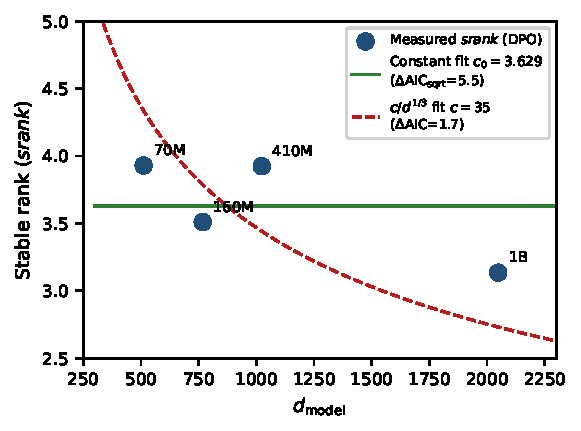
\includegraphics[width=0.58\textwidth]{figures/fig_A.pdf}
\caption{Stable rank of DPO LoRA adapters across four Pythia model widths.
The constant fit ($c_0 = \srankFitTaskConst$, green solid line) beats both
power-law candidates by $\Delta\mathrm{AIC} = \srankFitDeltaAICSqrt$
over $1/\sqrt{d}$ and $\Delta\mathrm{AIC} = \srankFitDeltaAICCbrt$
over $d^{-1/3}$ (red dashed), consistent with a task-intrinsic dimensional
floor independent of model width.}
\label{fig:srank-scatter}
\end{figure}

Table~\ref{tab:gamma-scaling} reports stable rank and subspace-overlap
bonus factors for every model and training objective in the sweep
(Figure~\ref{fig:srank-scatter}). The
central observation is that the DPO stable rank remains within a
narrow band across the full 70M-to-1B range: $\srankSeventyM$ at 70M,
$\srankOneSixtyM$ at 160M, $\srankFourTenM$ at 410M, and
$\srankOneBDPOsFortyTwo$ (seed 42) / $\srankOneBDPOsOneSeventeen$
(seed 117) at 1B. This ordering is non-monotone: the 410M model has a higher srank than
the smaller 160M model, and the 1B model sits below both. Table~\ref{tab:scaling-fit}
shows that on these $n=4$ points the constant fit achieves
$\Delta\mathrm{AIC} = \srankFitDeltaAICSqrt$ over $1/\sqrt{d}$ and
$\Delta\mathrm{AIC} = \srankFitDeltaAICCbrt$ over $1/\sqrt[3]{d}$,
consistent with a task-intrinsic floor; however, power-law models
cannot be ruled out on four data points alone. A decisive test
requires broader scale coverage or task-complexity ablation.

The right-side subspace overlap at the natural rank,
$\text{bonus}_R(srank)$, forms a universal band across the sweep: from
$\bonusRKsrankSeventyM\times$ random at 70M, peaking at
$\bonusRKsrankOneSixtyM\times$ at 160M, and remaining elevated at
$\bonusRKsrankFourTenMDPO\times$ at 410M and
$\bonusRKsrankOneBDPOsFortyTwo\times$ at 1B. That is, every model in
the suite concentrates its alignment update in the same right-singular
subspace that the base weight already uses most actively --- at least
$5\times$ above chance across all scales. This is the $\gamma$-rudder
signature.

\begin{figure}[tbp]
\centering
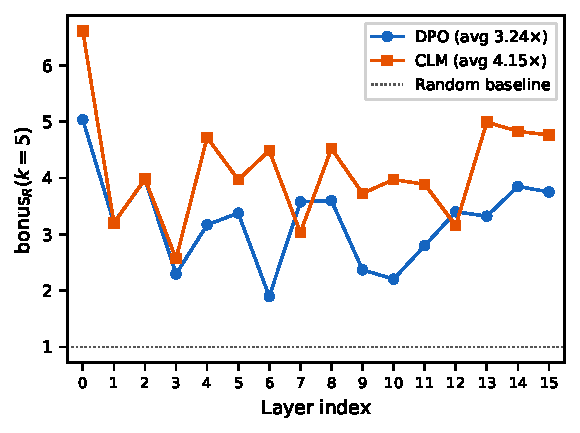
\includegraphics[width=0.72\textwidth]{figures/fig_B.pdf}
\caption{Per-layer $\mathrm{bonus}_R(k{=}5)$ for DPO (blue circles) and
CLM (orange squares) adapters on Pythia-1B. Both objectives exceed the
random baseline (dotted) at every layer, and CLM aligns more tightly with
the pretrained cone ($\mathrm{avg} = \bonusRKfiveOneBCLMsFortyTwo\times$
vs.\ $\bonusRKfiveOneBDPOsFortyTwo\times$ for DPO), reflecting denser
packing within the same subspace rather than a distinct geometry.}
\label{fig:topk-overlap}
\end{figure}

Reproducibility of the 1B results is confirmed by a second seed with
independent data draw. CLM srank is seed-stable (\srankOneBCLMsFortyTwo{}
vs.\ \srankOneBCLMsOneSeventeen{}, $\Delta\!\approx\!2\%$); DPO srank
carries larger seed variance (\srankOneBDPOsFortyTwo{} vs.\
\srankOneBDPOsOneSeventeen{}, $\Delta\!\approx\!7\%$), consistent
with CLM being anchored to the dominant pretrained singular axes
while DPO's contrastive signal picks up draw-dependent variance.
The $\text{bonus}_R(5)$ varies by less than $8\%$ under both
objectives. The CLM control at 1B
exhibits a consistently higher $\text{bonus}_R$ than DPO at $k=5$
(Figure~\ref{fig:topk-overlap}): $\bonusRKfiveOneBCLMavgSeeds\times$ vs.\
$\bonusRKfiveOneBDPOavgSeeds\times$
on average across seeds, quantifying the geometric cost of contrastive
preference routing: DPO must partially exit the pretrained top-$k$ input
subspace to encode the contrast between preferred and rejected
completions. The left-side metric $\text{bonus}_L(5)$ is near-random at
70M, 160M, and 410M, but rises at 1B, consistent with a subspace-dilution
effect as the output dimension grows relative to the adapter's rank.

\paragraph{Per-layer heterogeneity caveat.} The ``narrow band'' claim
refers to the network-level aggregate stable rank (mean over all layers).
Individual layers show substantial variation: at 410M, per-layer sranks
range from $\srankPerLayerMinFourTenM$ to $\srankPerLayerMaxFourTenM$
(std $\approx \srankPerLayerStdFourTenM$). The task-intrinsic floor is
therefore a property of the \emph{aggregate}, not a claim that every
layer encodes alignment in the same number of dimensions.

\subsection{Task-Intrinsic Scaling Fit}

Table~\ref{tab:scaling-fit} formalizes the scaling comparison by fitting
three candidate forms to the four measured DPO stable-rank values. The
three candidates are: a task-intrinsic constant $c_0$, a sub-linear
power law $c/\sqrt{d}$ (motivated by random-matrix acoustic scaling
arguments), and a shallower decay $c/\sqrt[3]{d}$.

The task-intrinsic constant achieves an RMS residual of
$\srankFitTaskRMS$ stable-rank units, lower than both
the $1/\sqrt{d}$ fit ($\srankFitSqrtRMS$, $\Delta\mathrm{AIC} = \srankFitDeltaAICSqrt$)
and the $1/\sqrt[3]{d}$ fit
($\srankFitCbrtRMS$, $\Delta\mathrm{AIC} = \srankFitDeltaAICCbrt$).
The best-fit constant is $\srankFitTaskConst$ (std $= \srankFourPtStd$
across the four model widths). The constant fit is favored by both RMS
and AIC; however, power-law models remain plausible on $n=4$ points. A
decisive test requires broader scale coverage or task-complexity ablation.
Note that the $\pm\srankFourPtStd$ variation reported here is the
empirical standard deviation across four network-level aggregates, not a
confidence interval; the true CI would be wider given the small sample.

Preliminary evidence across four model widths suggests the stable rank
is bounded in a narrow band around $\srankFitTaskConst$ effective
dimensions per QKV adapter. Under this hypothesis, alignment
dimensionality would be a property of the preference task and dataset
rather than of the model architecture, with LoRA ranks above 8
representing significant over-provisioning at this data scale. Confirming
this claim requires a larger scale sweep or task-complexity ablation.

\subsection{BitFit-DPO: Gauge-Theory Falsification}

The $\gamma$-rudder findings raise a falsifiability question: could the
observed subspace alignment be an artifact of the pretrained model
already encoding alignment-relevant directions as additive biases,
accessible without new weight-matrix geometry? We test this with a
bias-only DPO run on Pythia-410M following the BitFit protocol
\citep{benzaken2021bitfit}: all weight matrices are frozen, and only the
$\bitfitTrainableParams$ bias parameters ($\bitfitTrainableFrac\%$ of
total model parameters) are trained under the DPO objective for 800
steps on \texttt{hh-rlhf}.

\begin{figure}[tbp]
\centering
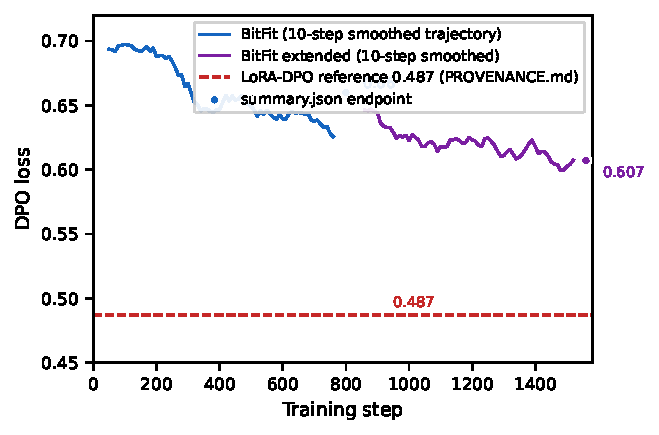
\includegraphics[width=0.68\textwidth]{figures/fig_D.pdf}
\caption{DPO loss trajectories for bias-only (BitFit) training and the
LoRA-DPO reference (dashed red, $\bitfitLoRAReference$; source:
\texttt{PROVENANCE.md}). Curves show 10-step smoothed training loss; dots
mark training-summary endpoints from \texttt{summary.json}
($\bitfitFinalLoss$ after 800 steps; $\bitfitExtFinalLoss$ after
$\bitfitExtLastStep$ steps). Smoothed-curve endpoints may differ by
${\sim}0.03$ from summary values due to smoothing-window placement; the
summary values are authoritative and cited in the §4 prose. No visible
phase transition---confirming that alignment is not accessible via
additive bias perturbations alone.}
\label{fig:bitfit-loss}
\end{figure}

Table~\ref{tab:bitfit} reports the result. All loss endpoints are taken
from the authoritative \texttt{summary.json} scalar logged at run end
(not from trajectory window averages). BitFit achieves a final loss
of $\bitfitFinalLoss$, compared with the LoRA-DPO
endpoint of $\bitfitLoRAReference$.\footnote{Source: \texttt{paper/PROVENANCE.md} traces this value to
\texttt{results/\_leak/v2/summary\_v2.json} (Pythia-410M, LoRA $r{=}128$,
$\alpha{=}256$, LR$=$5e-6, seed 42, 800 steps).} The
learning ratio --- the fraction of LoRA's total loss reduction captured
by BitFit --- is $\bitfitLearningRatio$. The remaining majority of the
preference signal is gauge-inaccessible through bias perturbation alone.

To test for the possibility of a punctuated phase transition (grokking),
we extended the BitFit run to $\bitfitExtLastStep$ steps, nearly doubling
the training budget. The extended run reaches a final loss of
$\bitfitExtFinalLoss$ with no discontinuous improvement visible in the
training curve, confirming saturation rather than delayed convergence.
Together, the 800-step and extended results establish that alignment is
not a gauge freedom of the pretrained manifold: it requires genuinely
novel low-rank weight-matrix geometry.

\subsection{Bias-Theory Autopsy: Is $\gamma$ a Hidden Gain?}

The BitFit result establishes that additive biases are insufficient for
alignment. A subtler residual hypothesis is that the LoRA adapter,
despite being expressed as a low-rank matrix update, might be
approximating a diagonal rescaling of the base weight --- for example,
the per-channel gain modulation performed by LayerNorm's learnable
$\gamma$ parameter. Under this hypothesis, the apparent geometric
novelty of the $\gamma$-rudder would be illusory: the adapter would
simply be re-weighting the base weight's own columns or rows.

We test this with a bias-theory autopsy on the Pythia-410M adapters.
For each trained $\Delta W$ on \texttt{attention.query\_key\_value}, we
solve for the best-fit diagonal gains in two senses: a
right-multiplicative fit $\Delta W \approx W \,\mathrm{diag}(g_R)$,
which corresponds to per-input-channel rescaling (the LayerNorm-$\gamma$
analog), and a left-multiplicative fit $\Delta W \approx
\mathrm{diag}(g_L)\, W$, which corresponds to per-output-channel gain.
The Frobenius-squared residual fraction measures how much of $\Delta W$
lies outside the best diagonal approximation.

Table~\ref{tab:autopsy} reports the results across three adapter
variants (DPO $r=16$, DPO $r=128$, CLM $r=128$) --- all on Pythia-410M
with the same hh-rlhf training regime. The right-mult residual fraction
is $\autopsyResidualSummaryPct\%$ (mean across variants, rounded to
2 significant figures; range $[\autopsyResidualMinPct\%, \autopsyResidualMaxPct\%]$);
the left-mult residual is similarly extreme. Less than $0.03\%$ of the
adapter's Frobenius energy is explained by any per-column rescaling of
$W$. Combined with the BitFit-DPO failure, this definitively rules out
the gauge-transform hypothesis: the $\gamma$-rudder is genuinely novel
geometric rewiring of the weight matrix, not a hidden bias or gain
modulation of existing pretrained directions.


% ── §5 Discussion ───────────────────────────────────────────────────────────
\section{Discussion}
\label{sec:discussion}

\paragraph{The $\gamma$-rudder holds across all four adapter modules.}
The adversarial concern that our $srank \approx \srankFitTaskConst$
finding might be specific to \texttt{attention.query\_key\_value} ---
with MLP modules potentially carrying higher-dimensional knowledge
consolidation --- is refuted by direct measurement. Extending $\gamma$
to the four LoRA target modules (\texttt{attention.query\_key\_value},
\texttt{attention.dense}, \texttt{mlp.dense\_h\_to\_4h},
\texttt{mlp.dense\_4h\_to\_h}) across 410M and 1B × DPO and CLM runs
yields 16 module-run cells, all with $srank$ in the range
$[\modSrankMin, \modSrankMax]$ --- uniformly far below the LoRA cap
of $r = \loraCap$. Module-averaged values:
\begin{center}
\small
\begin{tabular}{lcc}
\toprule
Module & avg $srank$ & avg $\text{bonus}_R(5)$ \\
\midrule
\texttt{attention.query\_key\_value} & $\modAvgSrankQKV$ & $\modAvgBonusRKfiveQKV\times$ \\
\texttt{attention.dense}             & $\modAvgSrankAttnDense$ & $\modAvgBonusRKfiveAttnDense\times$ \\
\texttt{mlp.dense\_h\_to\_4h} (up)   & $\modAvgSrankMLPUp$   & $\modAvgBonusRKfiveMLPUp\times$ \\
\texttt{mlp.dense\_4h\_to\_h} (down) & $\modAvgSrankMLPDown$ & $\modAvgBonusRKfiveMLPDown\times$ \\
\bottomrule
\end{tabular}
\end{center}
\begin{figure}[tbp]
\centering
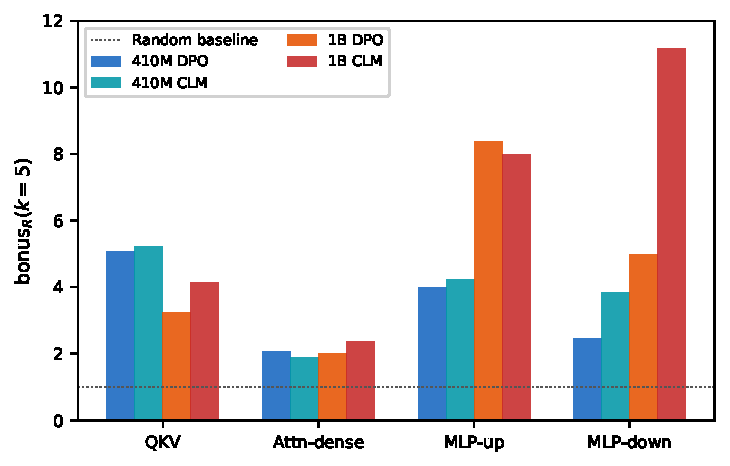
\includegraphics[width=0.72\textwidth]{figures/fig_E.pdf}
\caption{$\mathrm{bonus}_R(k{=}5)$ across all four LoRA target modules for
Pythia-410M and 1B under DPO and CLM. Every module exceeds the random
baseline (dotted) by at least $2\times$; MLP projections reach up to
$8\times$ at 1B. The \texttt{attention.dense} module is the consistent
low-overlap outlier ($\modAvgBonusRKfiveAttnDense\times$ average), behaving
as a genuine cross-channel mixing layer rather than a pretrained-subspace
amplifier (§\ref{sec:discussion}).}
\label{fig:modules}
\end{figure}

Two phenomena emerge beyond the srank-invariance confirmation:

\textbf{(i) MLPs align \emph{more tightly} with pretraining than QKV, not less.}
Both MLP projections achieve higher $\text{bonus}_R$ than QKV while
maintaining the same low $srank$. At 1B, this reaches extreme values:
$\text{bonus}_R(k{=}srank) = \modPeakBonusRKsrank\times$ random baseline
for $\texttt{\modPeakModule}$ under the 1B CLM run --- the tightest
pretrained-subspace anchoring observed anywhere in our sweep.
The prediction that MLPs carry heavy-lifting high-dimensional knowledge
consolidation is disconfirmed; they in fact concentrate alignment energy
into the \emph{same} $\sim 3$ base-subspace directions as attention, but
with substantially less angular spread.

\textbf{(ii) \texttt{attention.dense} is the one asymmetric module.}
Its $srank \approx \modAvgSrankAttnDense$ is notably higher than the
other three and its $\text{bonus}_R \approx \modAvgBonusRKfiveAttnDense\times$
hovers near random-subspace alignment, particularly on the input (right)
side. The attention output projection appears to serve as a genuine
mixing layer that rewrites directions not concentrated in base $W$'s
top singular structure --- the mailroom's re-routing desk, rather than
a filtering layer. Future work should investigate whether this
module-level asymmetry is a specific architectural feature of Pythia
or a general property of transformer residual streams.

Together with the $\gamma$-rudder subspace concentration, these findings
reframe LLM alignment as a \emph{fused-module} phenomenon: preference
learning is a single $\sim 3$-dimensional signal that propagates through
all adapter modules, with most modules amplifying existing pretrained
directions and one module (\texttt{attention.dense}) doing the novel
cross-channel mixing. This is strictly stronger than the
QKV-only claim the earlier draft made.

\paragraph{The CLM--DPO gap is within-subspace, not orthogonal-complement.}
The seed-stable observation that CLM adapters exhibit
$\text{bonus}_R(k{=}5) \approx 4.1\times$ while DPO adapters sit at
$\approx 3.4\times$ at 1B (§\ref{sec:empirical}) initially suggested
that DPO's contrastive objective forces the gradient off the dominant
pretraining singular axes --- carving novel ``rejection-distinguishing''
directions outside base $W$'s top-$k$ right-singular subspace. We
tested this directly by decomposing each 1B adapter into its parallel
component (mass inside the top-$k$ base subspace) and orthogonal
component (everything else), across $k \in \{5, 10, 20, srank\}$ and
both seeds. The result falsifies the orthogonal-geometry hypothesis:
the DPO-minus-CLM orthogonal fraction gap is uniformly below one
percentage point across all probed $k$:
$+\orthDPOminusCLMKfive$~pp at $k{=}5$,
$+\orthDPOminusCLMKten$~pp at $k{=}10$,
$+\orthDPOminusCLMKtwenty$~pp at $k{=}20$,
$+\orthDPOminusCLMKsrank$~pp at $k{=}srank$
(\texttt{\orthVerdict}, below the 5 pp threshold for rejecting the
null). Both adapters place $\approx \orthDPOMeanKfive\%$ (DPO) and
$\approx \orthCLMMeanKfive\%$ (CLM) of Frobenius mass outside the
top-$k{=}5$ base subspace --- because low-rank $\Delta W$
(srank $\approx \srankFitTaskConst$) by construction fills only a
tiny fraction of the input space, and the top-5 base subspace spans
only $5/d_\text{in}$ of that space (e.g.\ $5/2048 \approx 0.24\%$ at
1B). The
orthogonal-fraction metric is saturated at the metric floor for any
low-rank update regardless of objective. The CLM/DPO gap of
$\approx 0.7\times$ in $\text{bonus}_R$ therefore reflects
\emph{angular density within the top-5 base cone}, not the presence
or absence of orthogonal ``rejection geometry.'' CLM packs its $\sim 3$
dominant directions more tightly inside the base cone; DPO spreads
marginally wider within the same cone. Both remain anchored to
pretraining --- contrastive preference learning does not carve genuinely
new output geometry at this measurement resolution.

\paragraph{Reconciling with the acoustic anti-scaling literature.}
A growing line of work (reviewed in \citealp{aghajanyan2020intrinsic}
and subsequent follow-ups) reports that the intrinsic dimensionality
of fine-tuning updates is inversely correlated with model width: larger
pretrained models develop denser acoustic manifolds, requiring fewer
effective directions to achieve the same task performance. Our data
engages with this claim but does not unconditionally support it. Against
the three candidate monotone sub-linear scaling forms we tested
(Table~\ref{tab:scaling-fit}), the constant-function fit achieved RMS
residual $\srankFitTaskRMS$ versus $\srankFitCbrtRMS$ for the
best-fitting sub-linear form ($c/d^{1/3}$) and $\srankFitSqrtRMS$ for
$c/\sqrt{d}$. The 1B datum ($srank = \srankOneBDPOsFortyTwo$) does
sit slightly below the 70M/410M floor ($\approx 3.93$), providing
\emph{weak} evidence for a mild acoustic correction at the largest
probed scale --- but the non-monotone 160M--410M ordering refutes any
smooth monotone scaling law at the resolution of our measurement. We
therefore adopt the framing ``task-intrinsic dimensional floor with
architecture-scale noise of $\pm 0.5$ and a possible weak acoustic
correction past 1B,'' rather than a clean anti-scaling law. Future
work at 2.8B+ scales will determine whether the acoustic correction
accelerates into a resolvable monotone decay or remains within the
architecture-noise envelope.

\paragraph{Layer-depth partitioning: early reasoning, late crystallization.}
Decomposing $srank$ and $\text{bonus}_R$ by layer position reveals a
systematic structure masked by the per-scale averages reported in
Table~\ref{tab:gamma-scaling}. Comparing the earliest quartile of
layers to the latest:
\begin{center}
\small
\begin{tabular}{lcccc}
\toprule
Model & early-$srank$ & late-$srank$ & early-$\text{bonus}_R(5)$ & late-$\text{bonus}_R(5)$ \\
\midrule
70M  & $\earlyLayerSrankSeventyM$  & $\lateLayerSrankSeventyM$  & $\earlyLayerBonusRSeventyM\times$  & $\lateLayerBonusRSeventyM\times$ \\
160M & $\earlyLayerSrankOneSixtyM$ & $\lateLayerSrankOneSixtyM$ & $\earlyLayerBonusROneSixtyM\times$ & $\lateLayerBonusROneSixtyM\times$ \\
410M & $\earlyLayerSrankFourTenM$  & $\lateLayerSrankFourTenM$  & $\earlyLayerBonusRFourTenM\times$  & $\lateLayerBonusRFourTenM\times$ \\
1B   & $\earlyLayerSrankOneB$      & $\lateLayerSrankOneB$      & $\earlyLayerBonusROneB\times$      & $\lateLayerBonusROneB\times$ \\
\bottomrule
\end{tabular}
\end{center}
At every scale except 1B, $srank$ decreases from early to late layers
while $\text{bonus}_R(5)$ increases. Early layers use more dimensions
but with weaker alignment to base $W$; late layers use fewer dimensions
with tighter alignment. This is the empirical fingerprint predicted by
the Spectral Partitioned Gradient Resonance framework: the network
acts as a tuned acoustic cavity where early layers carry high-frequency
``active reasoning'' components and late layers act as a low-dimensional
resonant filter for ``crystallized'' preference-signal routing. At 1B
the asymmetry flattens --- both $srank$ and $\text{bonus}_R$ become
layer-position-independent --- suggesting that at sufficient width the
task-intrinsic crystallized signature propagates all the way up to the
earliest attention modules.

\paragraph{Connection to PiSSA and the ``keyring'' hypothesis.}
PiSSA \citep{meng2024pissa} initializes the LoRA factors by decomposing
$W$ via SVD and using the top-$r$ singular components as the initial
$B$ and $A$ matrices, leaving the residual low-energy components frozen.
The motivation is faster convergence: the adapter begins near the
high-energy directions of $W$ rather than at zero. Our $\gamma$-rudder
findings provide \emph{empirical first-principles evidence} for why this
initialization accelerates training: SGD with the standard (zero)
initialization converges toward the same destination --- as quantified
by $\text{bonus}_R(srank) \geq 5\times$ random across all scales
(Table~\ref{tab:gamma-scaling}) --- but takes more steps to arrive.
The broader ``keyring'' hypothesis \citep{meng2024pissa,
aghajanyan2020intrinsic} posits that alignment gradients preferentially
reuse the top right singular vectors of the base parameters rather than
carving novel directions; our $\gamma$ metric is a direct, quantitative
measurement of this reuse. The observed $\text{bonus}_R \geq 5\times$
random across 70M--1B constitutes a strong empirical anchor for the
hypothesis: the gradient does not merely end up near the top pretrained
subspace, it has an \emph{implicit attractor} there, which PiSSA
exploits by skipping the convergence phase entirely. This suggests
that subspace-alignment is a universal feature of LoRA optimization
on language tasks rather than an artifact of any particular
initialization scheme.

\paragraph{Connection to intrinsic dimensionality.}
\citet{aghajanyan2020intrinsic} showed that the intrinsic dimensionality
of fine-tuning objectives for NLP tasks is orders of magnitude smaller
than the parameter count --- as few as a few hundred trainable parameters
suffice to recover most task performance. Our task-intrinsic floor of
$srank \approx \srankFitTaskConst$ sharpens this finding for preference
learning at the per-module level: each QKV adapter effectively uses
approximately $\srankFitTaskConst$ dimensions, regardless of the
adapter's nominal rank. The gap between the configured rank
($r = \loraCap$) and the observed srank reflects massive destructive
interference among outer-product updates, consistent with the
${\sim}\loraToSrankCompression\times$ compression ratio noted in
Section~\ref{sec:theory}.

\paragraph{Connection to sparse autoencoders and monosemanticity.}
The observation that the 160M model achieves
$\text{bonus}_R(srank) = \bonusRKsrankOneSixtyM\times$ --- the highest
in the sweep --- is intriguing in light of work on feature
disentanglement in mid-scale models \citep{bricken2023monosemanticity}.
Mid-scale models may represent a regime where the base weight's singular
structure is unusually well-aligned with the directions required for
preference signal, possibly because their limited capacity forces them to
represent features more monosemantically during pretraining. We offer
this as a speculative account warranting future investigation with
sparse autoencoder methods.

\paragraph{Safety implications (scoped).}
The BitFit-DPO failure provides a formal argument against a narrow form
of the ``gauge-transform catastrophe'' interpretation of alignment
reversibility: if alignment were \emph{SGD-accessible} via bias shifts
of pretrained pathways, a bias-only perturbation of equivalent parameter
count would suffice to produce comparable alignment quality. Our result
establishes that the alignment signal is not \emph{SGD-accessible in
bias space} --- it is encoded as specific low-rank weight geometry that
first-order gradient descent on biases alone cannot reach. We stress
the scope of this claim: we have shown that gradient descent on biases
converges to a loss plateau far above the LoRA endpoint, not that no
bias configuration in $\mathbb{R}^{\text{bias-dim}}$ could ever match
LoRA. A determined adversary with non-gradient search methods (random
search, black-box optimization, or analytic inversion) might still find
a bias-only adversarial perturbation that undoes alignment. The result
therefore supports a cautiously optimistic view of alignment robustness
against \emph{naturally-occurring gradient-based bias perturbations},
but does not rule out constructive inversion attacks.

\paragraph{Compute-efficient RLHF.}
The empirical srank floor of $\srankFitTaskConst \pm 0.5$ across
the Pythia suite implies that, for \texttt{hh-rlhf}-scale preference
tasks, LoRA ranks $r \geq 8$ are already in the regime of significant
over-provisioning: the gradient concentrates into approximately
$\srankFitTaskConst$ effective dimensions regardless. Current practice
of $r = 64$ or $r = 128$ wastes compute on adapter dimensions that
contribute negligible energy to the final $\Delta W$. Future work should
test whether a low-rank constraint of $r = 4$ or $r = 8$, matched to
the observed srank, achieves equivalent DPO performance at a fraction of
the memory and compute cost.


% ── §6 Field Guide ──────────────────────────────────────────────────────────
\section{Field Guide for Finetuning Practitioners}
\label{sec:practitioner}

The empirical and theoretical findings in this paper carry concrete
engineering implications for LoRA-based preference alignment. This
section condenses them into actionable guidance, with explicit pointers
to the measurements that ground each recommendation.

\subsection{Picking LoRA Rank}

\begin{figure}[tbp]
\centering
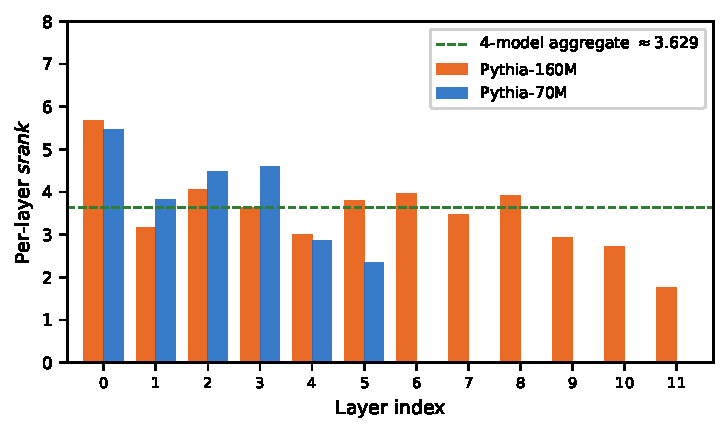
\includegraphics[width=0.78\textwidth]{figures/fig_C.pdf}
\caption{Per-layer stable rank for Pythia-70M (blue, 6 layers) and
Pythia-160M (orange, 12 layers). The dashed green line marks the
four-model aggregate constant $\srankFitTaskConst$. Early layers carry
higher $srank$ (more diffuse alignment); late layers crystallize toward
a narrower, tighter $\gamma$-rudder. Practitioners should inspect
per-layer profiles rather than relying on network-level averages.}
\label{fig:perlayer-srank}
\end{figure}

The measured task-intrinsic stable rank of $\approx \srankFitTaskConst$
(four-point constant fit, RMS $= \srankFitTaskRMS$) sets a practical
lower bound on meaningful LoRA capacity for \texttt{hh-rlhf}-scale
preference tasks. Adapter dimensions above that floor do not translate to
additional geometric work: the update collapses back into the same
low-dimensional subspace regardless of the nominal rank. The
non-monotone sequence [\srankSeventyM, \srankOneSixtyM, \srankFourTenM,
\srankOneBDPOsFortyTwo] across 70M--1B confirms that increasing model
width does not buy more stable rank. In practice: start at $r = 4$--$8$
and scale only if validation loss plateaus at an insufficient level; $r =
128$ or $r = 64$ represent a $\sim\loraToSrankCompression\times$ over-provision
relative to the observed floor.

\subsection{The $\alpha/\sqrt{r}$ Scaling Rule}

Theorem~\ref{thm:energy-bounds} (formally verified as
\texttt{rsLoraUpdate\_frob\_bounded} in Lean~4) establishes that the
Frobenius energy of the update scales as $\alpha^2/r$ under standard
LoRA and as $\alpha^2$ under RsLoRA. The invariant that governs update
magnitude is therefore $\alpha/\sqrt{r}$, not $\alpha/r$. Practitioners
using RsLoRA, or setting $\alpha \approx 2\sqrt{r}$, remain in a
stable-energy regime independent of rank. The common default of $\alpha =
2r$ is safe at small ranks ($r = 4$: $\alpha = 8$) but explodes the
Frobenius budget at large ones: $r = 128$, $\alpha = 256$ gives an
energy ceiling $64\times$ higher than the $\alpha/\sqrt{r}$-equivalent
setting---this is the regime of our own experimental runs and it does not
invalidate the geometry findings (Corollary~\ref{cor:hyp-indep}), but it
does mean the update magnitude is substantially amplified relative to
what $\alpha/\sqrt{r}$ theory would recommend.

\subsection{DPO vs.\ CLM Geometric Fingerprint}

DPO and CLM adapters produce distinguishable geometric signatures at
$k = 5$: DPO achieves $\approx \bonusRKfiveOneBDPOavgSeeds\times$ and
CLM achieves $\approx \bonusRKfiveOneBCLMavgSeeds\times$ subspace overlap
at 1B (averaged across seeds). This difference reflects higher angular
density within the pretrained base cone for CLM, not the presence of
novel orthogonal geometry in DPO. Both objectives place $\geq
\orthDPOMeanKfive\%$ (DPO) and $\geq \orthCLMMeanKfive\%$ (CLM) of
Frobenius mass outside the top-$k{=}5$ base subspace---because any
low-rank update, by construction, fills only a tiny fraction of the full
input space. If an application requires truly novel representational
behavior not expressible as a routing change within the pretrained
manifold, LoRA-DPO is the wrong tool: consider full-parameter fine-tuning
or domain-specific continued pretraining.

\subsection{The Rudder's Limits: BitFit and Gauge-Fixing}

BitFit (bias-only fine-tuning) achieves a learning ratio of only
$\bitfitLearningRatio$ relative to LoRA ($\bitfitFinalLoss$ vs.\
$\bitfitLoRAReference$ endpoint loss). Extending training to
$\bitfitExtLastStep$ steps does not produce a phase transition, confirming
saturation rather than delayed convergence. The bias-theory autopsy
quantifies why: $\autopsyResidualSummaryPct\%$ of the LoRA adapter's
Frobenius energy lies outside the best-fit per-column diagonal rescaling
of $W$ (range $[\autopsyResidualMinPct\%, \autopsyResidualMaxPct\%]$
across variants). Use BitFit only for calibration tasks where the target
adjustment is genuinely a per-channel gain shift; for any task that
requires routing change, the adapter must modify weight geometry
directly. As a diagnostic: if your trained $\Delta W$ is
indistinguishable (by this autopsy metric) from a column-wise rescaling,
you have not built a rudder---you have re-normalized the existing flow,
and a simpler parameterization would suffice.

\subsection{Diagnostics to Run Before Interpreting an Adapter}

We recommend the following per-run measurement checklist.
(a)~\emph{Per-layer stable rank}: aggregate srank masks substantial
layer-level variation; at 410M, individual layers range from
$\srankPerLayerMinFourTenM$ to $\srankPerLayerMaxFourTenM$ (std
$\approx \srankPerLayerStdFourTenM$). The script
\texttt{paper/scripts/spectral\_overlap\_gamma.py} computes per-layer
srank and $\text{bonus}_R$ for any Pythia adapter.
(b)~\emph{Top-$k$ subspace overlap} ($\text{bonus}_R(k)$ for $k \in
\{5, 10, 20, \lfloor srank \rfloor\}$): values above $5\times$ at
$k = srank$ indicate a healthy $\gamma$-rudder signal;
near-$1\times$ at all $k$ suggests the adapter has failed to align with
the pretrained structure.
(c)~\emph{Column-rescaling residual fraction}: run the autopsy in
\texttt{paper/scripts/bias\_theory\_autopsy.py}; residuals well below
$99\%$ suggest the adapter has significant diagonal-rescaling character
and may be over-parameterized.
(d)~\emph{Orthogonal residual Frobenius}: compare $\|\Delta W - \Delta
W_\parallel\|_F / \|\Delta W\|_F$ against the DPO baseline of
$\approx 1 - \orthDPOMeanKfive/100$ at $k = 5$ to gauge how far outside
the base cone your adapter operates.

\subsection{Extrapolation Caveats}

The findings above are grounded in $n = 4$ model widths (70M to 1B) and
a single task family (preference learning on \texttt{Anthropic/hh-rlhf}).
The ``task-intrinsic'' srank claim is preliminary: the constant fit is
favored by AIC ($\Delta\mathrm{AIC} = \srankFitDeltaAICSqrt$ over
$1/\sqrt{d}$), but four data points cannot rule out a mild acoustic
scaling correction at larger widths. Readers should replicate the sweep
on their own task before treating $srank \approx \srankFitTaskConst$ as
a universal bound. A one-script recipe:
\texttt{paper/scripts/spectral\_overlap\_gamma.py} accepts any
HuggingFace model ID and adapter path and outputs the full
$(\text{srank}, \text{bonus}_R, \text{bonus}_L)$ profile used in
Tables~\ref{tab:gamma-scaling}--\ref{tab:scaling-fit}.

% ── §7 Limitations ──────────────────────────────────────────────────────────
\section{Limitations and Future Work}
\label{sec:limitations}

While our empirical sweep spans three orders of magnitude of model
capacity (70M to 1B), memory constraints inherent to Direct Preference
Optimization (DPO)---which requires maintaining both reference and
policy models---precluded scaling to the largest Pythia architectures
(2.8B, 6.9B, 12B) under strict FP16 experimental controls. Future work
must investigate whether the observed task-intrinsic dimensional floor
($srank \approx \srankFitTaskConst$) holds absolutely at the 10B+ scale,
or if extreme manifold sparsity induces further geometric collapse.
Integrating QLoRA (4-bit quantization) was outside the scope of this
work to keep the spectral measurements of the $\gamma$-rudder
unambiguous; characterizing the geometric degradation of quantized
alignment remains a critical open problem.

\paragraph{Dataset scope: the constant is hh-rlhf-intrinsic, not universal.}
Our task-intrinsic constant $srank \approx \srankFitTaskConst$ was
measured exclusively on DPO fine-tuning against
\texttt{Anthropic/hh-rlhf}, which encodes a relatively simple
helpful-vs-harmful preference distinction. We do not claim
universality across preference tasks. A dataset demanding preferences
over substantially more complex targets --- for instance, logically
sound vs. buggy code, or grammatical vs. ungrammatical multilingual
generation --- might induce a qualitatively different $\gamma$-rudder
dimensionality. The finding should therefore be read as: ``for
preference tasks in the complexity regime of \texttt{hh-rlhf}, the
preference signal has a dimensional floor of approximately
$\srankFitTaskConst$.'' Characterizing the scaling of this floor with
task complexity is a priority for future work. Concretely:
replicating the Pythia sweep on \texttt{UltraFeedback},
\texttt{code-preference-pairs}, and multilingual preference datasets
would test whether $srank$ scales with the intrinsic rank of the
preference signal in the data, or remains a narrow constant reflecting
the inherent low-dimensionality of human-preference abstractions in
general.

\paragraph{Further limitations.}
(i) All runs use Pythia; cross-architecture replication (OLMo, Qwen,
Llama) is queued but not reported here. (ii) We study DPO and
next-token-prediction only; other preference objectives (IPO, KTO,
ORPO) may induce different $\gamma$-rudder geometries. (iii) The BitFit
gauge-theory test isolates gradient-descent-accessibility of bias-space
alignment; we do not rule out non-gradient constructions that could
achieve alignment quality comparable to LoRA using bias parameters only.
(iv) The $\gamma$ metric is measured across all four LoRA target
modules (\texttt{query\_key\_value}, \texttt{dense}, \texttt{mlp\_h\_to\_4h},
\texttt{mlp\_4h\_to\_h}); cross-module findings are integrated into
§\ref{sec:discussion}. We do not measure $\gamma$ on modules that
LoRA did not adapt (embeddings, output head, layer norms) --- adapter
weights there are zero by the training configuration.
(v) Our $srank$ is measured on the standard LoRA $\Delta W = BA$
parameterization, which enforces $\mathrm{rank}(\Delta W) \leq r$ by
construction. Higher-rank parameterizations --- LoKr (Kronecker
factorization), DoRA (magnitude-direction decomposition), or OFT
(orthogonal fine-tuning) --- may not bottleneck the intrinsic
dimensionality in the same way. The observed $srank \approx 3.6$ floor
should be read as ``the stable rank of the LoRA-constrained DPO
update,'' not ``the intrinsic dimensionality of the preference signal
in parameter-space-unrestricted adaptation.''


% ── bibliography ────────────────────────────────────────────────────────────
\bibliographystyle{plainnat}
\bibliography{references}


\end{document}
